\documentclass{alex_hü}

\name{Alexander Helbok}
\course{Grundpraktikum}
\hwnumber{1}


\begin{document}

\begin{mybox}{Analyse}
	\begin{wrapfigure}[100]{r}{0.5\textwidth}
		\centering
		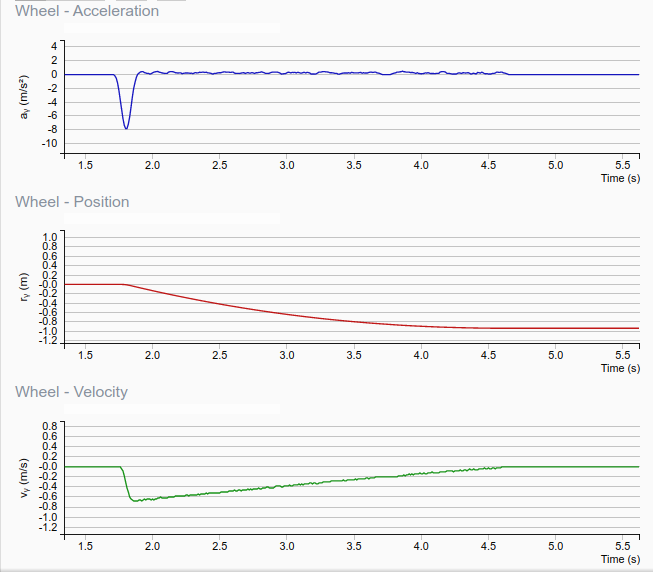
\includegraphics[width=0.5\textwidth]{Versuch 1 - 3}
	\end{wrapfigure}
	In der nebenstehenden Abbildung sieht man jeweils den Ort, die Geschwindigkeit und die Beschleunigung des IOLab Messgeräts auf die Zeit aufgetragen. Der oberste Plot zeit die Position in Bezug auf die Anfangslage, der grüne Graph zeigt die Geschwindigkeit des Geräts und in blau sieht man die beschleunigung in Bewegungsrichtung.
%
\end{mybox}

\end{document}